\section{IntelliJ IDEA}
\author{Benjamin Besic}

IntelliJ IDEA ist eine der führenden Entwicklungsumgebungen für die Programmiersprache Java. Sie wurde vom Unternehmen Jetbrains im Jahre 2000 entwickelt.
\\* Außerdem bietet sie ebenfalls Entwicklungsmöglichkeiten für Kotlin, Groovy, Scala und auch Android.
 Sie ist immer auf dem neusten Entwicklungsstand, wird laufend mit Updates versorgt und unterstützt die derzeit gängigen Programmiertools
wie Docker, Kubernetes, Maven, Datenbank-Tools, Git, Jakarta EE und viele weitere.
Es gibt eine kostenpflichtige Ultimate Version und eine Community Version, die kostenfrei zur Verfügung gestellt wird.
\\* IntelliJ zeichnet auch die Anzahl an Erweiterungen mittels Plugins aus. Die Umgebung besitzt auch eine
sehr intuitive Intelligenz, die es dem Entwickler sehr einfach macht damit zu programmieren.
\cite{IntJ} \\*
Wir haben uns dafür entschieden, da wir damit viel Erfahrung hatten und die oben genannten Punkte
unterstützten unsere Entscheidung enorm.

\section{Git}
\author{Benjamin Besic}
Git ist ein Versionskontrollsystem (oft abgekürzt durch VCS) für Entwickler. Es ist ein Open-Source System, das im Jahre 2005
von Linus Torvald entwickelt wurde. Laut einer Stack Overflow-Umfrage von Entwicklern nutzen über 87 \% der Entwickler Git.
\cite{GitKinsta}
\\* Zu aller erst muss man den Begriff Versionskontrolle erklären, um Git zu verstehen.
\subsection{Versionskontrolle}
Diese dient dazu, um den originalen Quellcode effizient mit mehreren Personen editieren bzw. entwickeln zu können. 
\\* Die Entwickler arbeiten mit Verzweigungen und Zusammenführungen. Jeder Entwickler kann Änderungen sicher durchführen, ohne seine Kollegen dabei 
zu behindern. Diese Änderungen können dann, sobald sie funktionsfähig sind, wieder in den Hauptquellcode eingebunden werden.
Alle Änderungen sind zurückzuverfolgen und bei Bedarf kann man sie dann wieder zurücksetzen.
\cite{GitKinsta} \\*

\subsection{Git Funktionsweise}
Jeder Entwickler hat seine eigene Version des Projekts (Working Directory), die er frei bearbeiten kann. Diese bekommt man durch einen Klon des Projekts (\hyperref[sec:Clone]{Clone}). \\* Diese Änderungen kann man aufteilen und 
in Paketen bereitstellen, nach dem man diese durch Commits trennt. Einen \hyperref[sec:Commit]{Commit} kann man benennen. \\*
Diese Commits kann man dann online veröffentlichen durch einen \hyperref[sec:Push]{Push}. Ein Push ist nur möglich, wenn man die aktuellste Version des Projekts
auf seinen Rechner gezogen hat (\hyperref[sec:Pull]{Pull}). 
Einem Push kann man einen bestimmten Zweig (\hyperref[sec:Branch]{Branch}) zuordnen. 
\begin{figure}[htp]
    \author{David Ignjatovic}
    \centering
    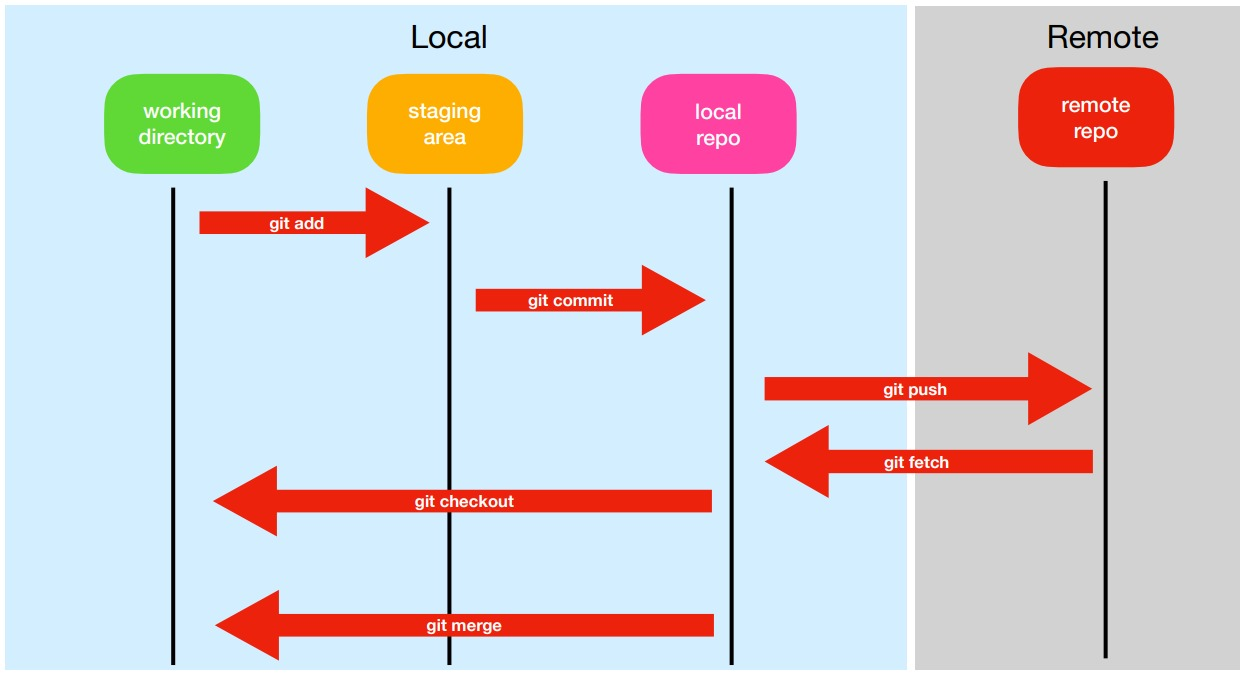
\includegraphics[scale=0.35]{pics/GitWorkflow.jpg}
    \caption{Darstellung des Git Workflows}
    \label{fig:impl:GitWorkflow}
\end{figure}
Diese Zweige dienen dazu, um das Projekt in verschiedene
unabhängige Teile zu trennen, falls man zum Beispiel an einer Demo Version weiterschreiben möchte. \\* Nach einem erfolgreichen Push sind die Änderungen
online auf dem Repository zu finden. Ein Repository ist der "Ordner", wo alle Dateien online gespeichert zu finden sind. 
\\* Ein Vorteil, den Git ebenfalls bietet ist das jeder Commit eine Version des Projekts ist, die man bis zum Zeitpunkt vom Commit herunterladen oder klonen kann.
Jedes Projekt kann privat oder öffentlich gemacht werden, sodass auch Personen, die keine Entwickler sind, darauf zugreifen können.
\cite{GitExpl} 



\subsection{Git Befehle}

\subsubsection{Clone}
\label{sec:Clone}
Es initialisiert ein Git Repository auf dem Rechner und ladet die zugehörigen Dateien runter.
Wenn man es nicht spezifisch angibt, klont es den Master Branch. Der Master Branch ist der Hauptzweig, eines jeden Git Projekts.
Innerhalb des erstellten Ordners können alle weiteren Git Befehle ausgeführt werden. \cite{GitCmnds}
\subsubsection{Commit}
\label{sec:Commit}
Ein Commit beschreibt Änderungen, die man im Projekt gemacht hat. Jeder Commit hat eine Bezeichnung, mit der der Entwickler die Änderungen,
die er gemacht hat beschreiben kann. Zu jedem Commit gehören auch die Dateien die dabei geändert bzw. hinzugefügt wurden.
\\* Es speichert den Zustand des gesamten Projekts bis zu dem Zeitpunkt und kann danach jederzeit abgerufen oder rückgängig gemacht werden.
Diese Änderungen bleiben aber zunächst nur lokal auf dem Rechner. \cite{GitCmnds}

\subsubsection{Push}
\label{sec:Push}

Ein Push dient dazu, um die lokalen Änderungen (Commits) zu veröffentlichen. Es kopiert den aktuellen, lokalen Stand und speichert diesen auf 
das vom Internet erreichbare Repository. \\* Einem Push kann ein Zweig (Branch) zugeordnet werden um die Änderungen zuzuordnen. 
Ansonsten wird der Master Branch genommen. \cite{GitCmnds}

\subsubsection{Pull}
\label{sec:Pull}
Der Pull Befehl kopiert die Inhalte vom öffentlichen Repository und fasst diese mit den lokalen Zustand auf dem 
rechner zusammen (merge). Es dient dazu die aktuelle Version des Projekts auf den Rechner herunterzuladen.
\\* Falls es Konflikte zwischen der derzeitigen und neusten Version gibt, werden die Änderungen zusammengeführt. \cite{GitCmnds}

\subsubsection{Branch}
\label{sec:Branch}
Die Branch Befehle dienen dazu um eine neue Abzweigung des Projekts (Branch) zu erstellen.
\\*
Branches erstellt man, wenn man an einer neuen Version des Projekts arbeitet und diese vom Hauptteil trennen will.
Meistens werden dadurch neue Funktionen programmiert, die später wieder in den Master Branch eingebunden werden.
\\* Der Vorteil daran ist, dass man an neuen Funktionalitäten experimentieren kann, ohne den Hauptentwicklungsstand zu 
beeinflussen. Branches können jederzeit gelöscht oder wieder ins Hauptprojekt integriert werden.
Es kann simultan am Master Branch und an Nebenzweigen gearbeitet werden durch trennen mit dem Push Befehl. \cite{GitExpl}

\begin{figure}[htp]
    \author{David Ignjatovic}
    \centering
    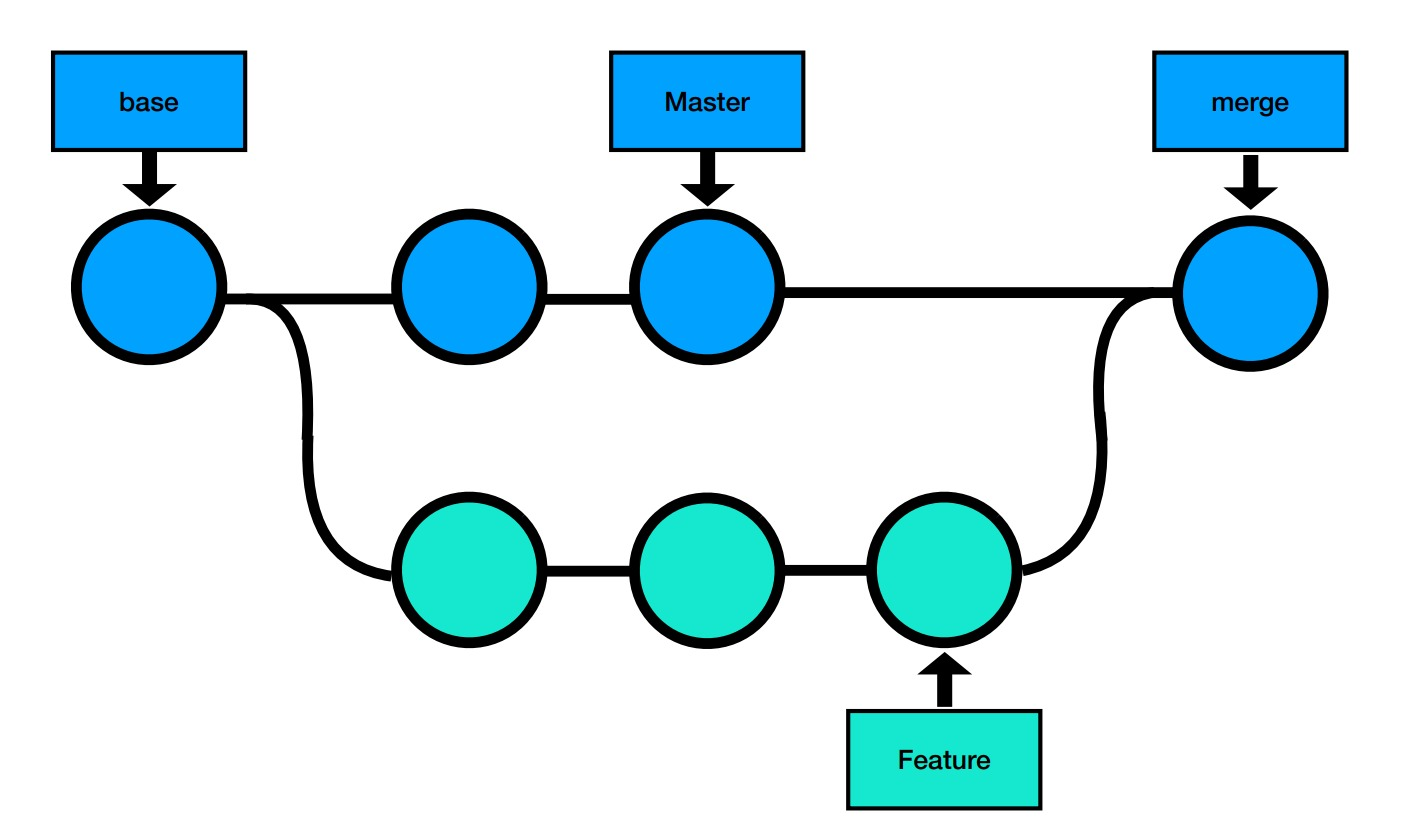
\includegraphics[scale=0.3]{pics/GitBranches.jpg}
    \caption{Darstellung von Branches in einem Repository}
    \label{fig:impl:GitBranches}
\end{figure}

\subsection{GitHub}
GitHub ist ein gewinnorientiertes Unternehmen, dass einen auf Cloud basierten Git Repository Hosting-Service anbietet.
Es wurde im Februar 2008 gestartet und von Chris Wanstrath, PJ Hyett, Scott Chacon und Tom Preston-Werner entwickelt.
Es ist das beliebteste Tool um Softwareprojekte zu verwalten und wird von über 73 Millionen Entwicklern und über 4 Millionen Organisationen
benutzt. Dazu ist es das größte und am meisten fortgeschrittene Entwicklungssystem, das es gibt. \cite{GitHub} \\*
Es vereinfacht die Nutzung von Git für Teams und auch Einzelpersonen. 
Jeder kann sich einen GitHub Account erstellen und direkt loslegen und seine Arbeiten auf Repositories veröffentlichen.
Es ist nicht nur zwingend für Code-basierte Projekte verwendbar sondern auch Websiten erstellen und das Schreiben von Büchern ist möglich.
\\*
Was GitHub ausmacht ist die Benutzerfreundlichkeit und die Integration von Git. Außerdem bietet Github viele andere Funktionen wie zum Beispiel ein Projekt Board an,
was es erleichtert innerhalb eines Teams, Probleme besser lösen zu können. \\*
Es gibt ebenfalls bezahlte Pläne, die es vor allem Organisationen und Unternehmen leichter macht Unternehmensprojekte zu verwalten durch zusätzliche Funktionen.
\cite{GitKinsta}



\section{Java}

\section{Java EE}

\section{Maven}

\subsection{Java EE vs. Quarkus}

\subsection{JPA}

\subsection{Hibernate}

\subsection{Panache}

\section{JBoss}

\section{Cypress}

\section{Keycloak}
\author{Benjamin Besic}

\section{Oracle Datenbank}

\section{Vue.js}
\author{Benjamin Besic}
Vue.js ist ein JavaScript-Webframework, das zum Erstellen von Single-Page-Webanwendungen dient. 
Es wurde von einem kleinen Team im Jahre 2014 entwickelt mit dem ursprünglichem Autor Evan You.\\* Vue ist relativ neu und die große Stärke
von Vue ist die einfache Lernkurve, die Vielseitigkeit und die Leichtgewichtigkeit. Man benötigt Kenntnisse in JavaScript, HTML, CSS und schon kann man loslegen
mit deren ausführlich dokumentierten Guide\cite{VueGuide}. \cite{VueWissen} \cite{VueWiki}\\*

\subsection{Vue Funktionsweise}

\subsubsection{Model-View-Viewmodel (MVVM) Pattern }
Vue.js benutzt das MVVM Pattern. Das Pattern trennt die Darstellung von der Logik der Benutzer-UI's.
Dazu ist ein Datenbindungsmechanismus vorausgesetzt. Dadurch können sich Entwickler und Interfacedesigner trennen und ihre Aufgaben im Projekt 
aufteilen. \\*
Dieses Pattern wurde 2005 von John Gossman veröffentlicht. \cite{MVVM}

\begin{figure}[htp]
    \centering
    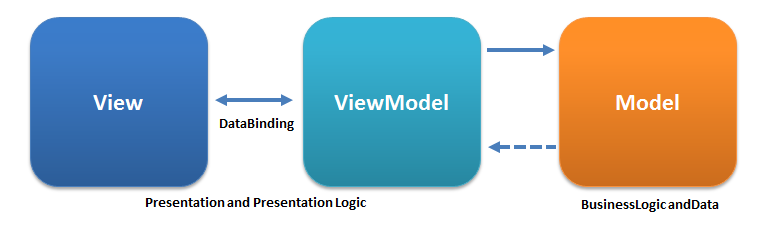
\includegraphics[scale=0.7]{pics/MVVMPattern.png}
    \caption{Darstellung von Branches in einem Repository}
        \small \url{https://upload.wikimedia.org/wikipedia/commons/8/87/MVVMPattern.png}
    \label{fig:impl:MVVM}
\end{figure}

\begin{itemize}
    \item \textbf{View:} Enthält alle Elemente die durch die Benutzeroberfläche angezeigt werden. Es bindet sich an das ViewModel, welches die Eigenschaften der View bestimmt.
    \item \textbf{ViewModel:} Es enthält die Logik des UI's. Es tauscht sich mit dem Model aus und benützt seine Methoden und Dienste. Gleichzeitig
          gibt es der View Eigenschaften, die dem Model entsprechen. Es bindet Daten mit der View und sich selbst (DataBinding).
    \item \textbf{Model:} Diese Schicht enthält alle Daten die der Benutzer manipuliert oder aufruft. Es enthält die gesamte Geschäftslogik.\cite{MVVM}
\end{itemize}

\clearpage

\subsubsection{Vue Instance}

Jede Vue Applikation beginnt mit der Erstellung einer Vue Instanz.

\begin{lstlisting}[language=JavaScript,caption=Vue Instanz,label=lst:impl:foo]
    var vm = new Vue({
        // options
    }) 
\end{lstlisting}

Die Variable vm steht für ViewModel, was unsere Vue Instanz darstellt. Man kann jeder Instanz Optionen zuweisen, um sie zu konfigurieren.
Diese Instanz wird auch als Root Instanz bezeichnet und bildet den Stamm eines Baumes mit Komponenten. 

\begin{figure}[htp]
    \centering
    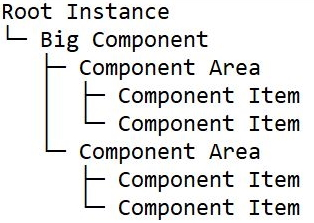
\includegraphics[scale=1]{pics/RootComponentTree.JPG}
    \caption{Der Stammbaum einer Root Instanz}
    \label{fig:impl:RootComponentTree}
\end{figure}
Zu einer Instanz gehört auch der data-Bereich. Dieser beherbergt alle Properties einer
Instanz und diese Properties reagieren auf Veränderungen im Code. Noch dazu kann jede Instanz Methoden haben. \\*
Jede Instanz hat auch seine Lifecycle Hooks, dies sind Methoden, die zu bestimmten Zeitpunkten einer Instanz ausgeführt werden. \cite{VueGuideInstance}
Diese sind:
\begin{itemize}
    \item \textbf{created}
    \item \textbf{mounted}          
    \item \textbf{updated} 
    \item \textbf{destroyed} 
\end{itemize}
\clearpage

\subsubsection{Lifecycle Diagram}
Das Diagramm hier stellt den Ablauf einer Erstellung einer neuen Vue Instanz dar.

\begin{figure}[htp]
    \centering
    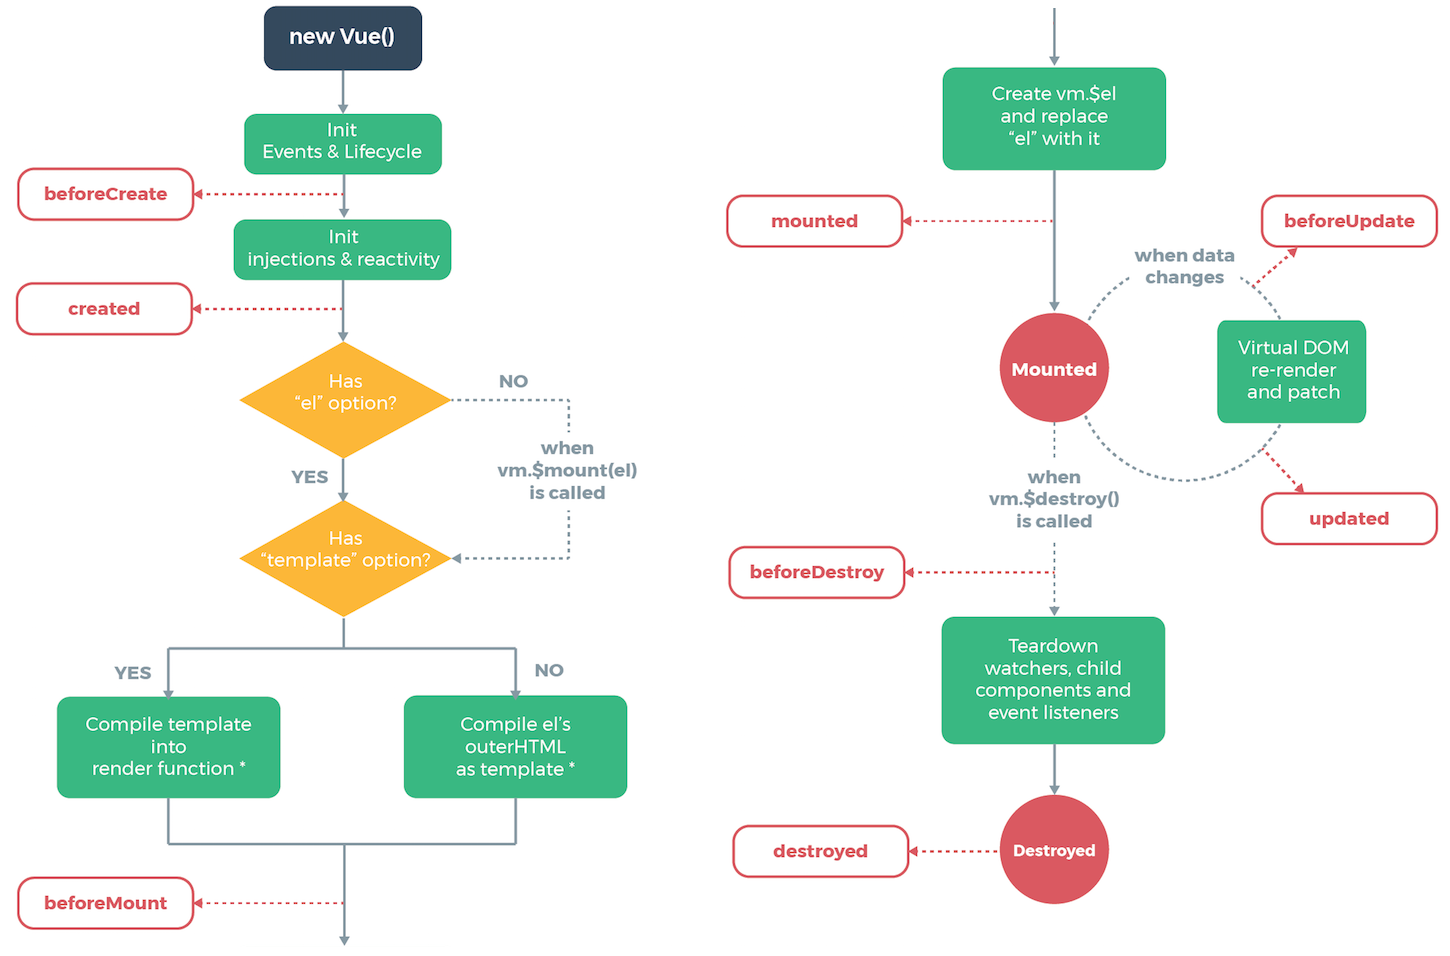
\includegraphics[scale=0.3]{pics/VueInstanceLifeCycle.png}
    \caption{Diagramm des Ablaufs einer Vue Instanz}
        \small \url{https://www.oreilly.com/library/view/full-stack-vuejs-2/9781788299589/assets/9f308e86-bbbe-489c-9f93-06abe2675081.png}
    \label{fig:impl:VueInstanceLifeCycle}
\end{figure}


\subsubsection{Vue Components}
Komponenten sind wiederverwendbare Vue Instanzen mit einem eigenen Namen. Diese Komponenten können mittels HTML-Tags in anderen Komponenten verwendet werden.


\section{Angular vs. Vue}

\section{HTML}

\section{CSS}

\section{Javascript}

\section{Json Web Token (JWT)}

\section{Progressive Web App(PWA)}

\section{Google Charts}

\subsubsection{Deepest}
Vermeide mich.